\documentclass{article}
\usepackage{graphicx}
\title{Calculus Third Edition Problems Solutions}
\author{Henrik Samuelsson}
\setcounter{section}{-1}

\begin{document}
\maketitle
Solutions to problems from the book Calculus Third Edition written by Professor Gilbert Strang.
\section{Highlights of Calculus}
\subsection{Distance and Speed // Height and Slope}
\subsubsection{Practice Questions Solutions}
\begin{enumerate}
    \item A graph of a function $f(t)$ that goes up and down and up again is draw to the left in the below figure. And then to the right another graph showing the corresponding slope of the first graph.
    \begin{figure}[h]
        \caption{Caption for my figure}
        \centering
        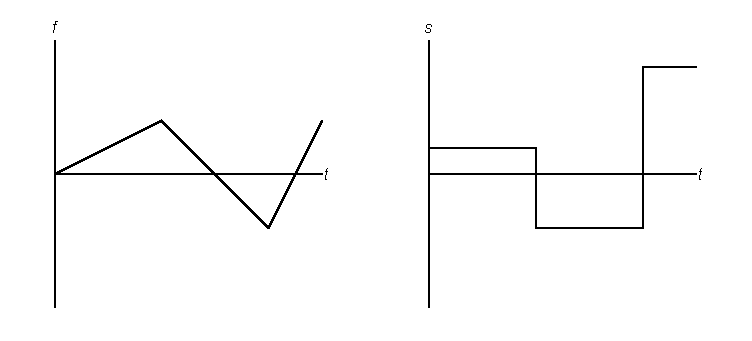
\includegraphics[width=0.75\textwidth]{slopes.pdf}
      \end{figure}
\end{enumerate}
\end{document}